\documentclass{beamer}
%
% Choose how your presentation looks.
%
% For more themes, color themes and font themes, see:
% http://deic.uab.es/~iblanes/beamer_gallery/index_by_theme.html
%
\mode<presentation>
{
  \usetheme{default}      % or try Darmstadt, Madrid, Warsaw, ...
  \usecolortheme{crane} % or try albatross, beaver, crane, ...
  \usefonttheme{structurebold}  % or try serif, structurebold, ...
  \setbeamertemplate{navigation symbols}{}
  \setbeamertemplate{caption}[numbered]
} 

\usepackage[english]{babel}
\usepackage[utf8x]{inputenc}
\usepackage{listings}

\title[ML]{Machine Learning}
\author{Pawel Wocjan}
\institute{University of Central Florida}
\date{Spring 2019}

\begin{document}

\begin{frame}
  \titlepage
\end{frame}

\begin{frame}[fragile]{Validation set}

\begin{itemize}
\item We introduced previously the partitioning a data set into a training set and a test set. 
\item This partitioning enabled you to train on one set of examples and then to test the model against a different set of examples. 
\item With two partitions, the workflow would look as follows:
\end{itemize}

{\footnotesize
\begin{verbatim}
     Train model on Training Set --> Evaluate model on Test Set
            ^                                            |
            |                                            |
            +---------- Tweak model according <----------+
                        results on Test Set
                                 |
                                 V
                         Pick model that does best
                         on Test Set
\end{verbatim}
}
\end{frame}

\begin{frame}{Validation set}
\begin{itemize}
\item Dividing the data set into two sets is a good idea, but it is not enough. 
\item You can greatly reduce the chances of overfitting by partitioning the data into three subsets shown below:

\medskip
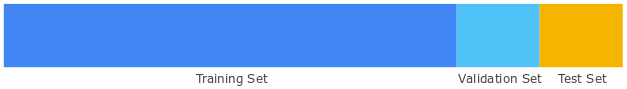
\includegraphics[width=0.9\textwidth]{images/PartitionThreeSets.png}

\item Use the validation set to evaluate results from the training set. 
\item Then, use the test set to double-check your evaluation after the model has ``passed'' the validation set.
\end{itemize}
\end{frame}

\begin{frame}[fragile]{Validation set}
\begin{itemize}
\item With three partitions, the workflow looks as follows:
\end{itemize}
{\footnotesize
\begin{verbatim}
Train model on Training Set --> Evaluate model on Validation Set
   ^                                                       |
   |                                                       |   
   +---------------- Tune model according <----------------+ 
                     results on Validation Set
                            |
                            V
               Pick model that does best --> Confirm model 
               on Validation Set             on Test Set
\end{verbatim}
}
\begin{itemize}
\item In this improved workflow:
\begin{itemize}
\item Pick the model that does best on validation set.
\item Double-check that model against the test set.
\end{itemize}
\item This is a better workflow because it creates fewer exposures to the data set.
\end{itemize}
\end{frame}

\begin{frame}{Validation methods}
\begin{itemize}
\item Splitting your data into
\begin{itemize}
\item training set
\item validation set
\item test set
\end{itemize}
may seem straightforward, but there are a few advanced ways to do it. 
\item This is especially important when there is little data available.
\end{itemize}
\end{frame}

\begin{frame}[fragile]{Simple hold-out validation}
\begin{itemize}
\item Set apart some fraction of your data as your test set.
\item Train on the remaining data, and evaluate at the end on the test set.
\item To prevent information leaks, you shouldn't tune your model based on the test set, and therefore you should also reserve a validation set.
\item Schematically, hold-out validation look as follows:
\end{itemize}
\begin{verbatim}
+-------------------------------------------+
|                              | Held-out   |
|          Training set        | validation |
|                              | set        |
+-------------------------------------------+
\end{verbatim}
\end{frame}

\begin{frame}[fragile]{Pseudo code for simple hold-out validation}
\vspace{-0.75cm}
\begin{lstlisting}
# split non-test data into training and validation data

training_data = data[num_validation_samples:]
validation_data = data[:num_validation_samples]

model = get_model()
model.train(training_data)

validation_score = model.evaluate(validation_data)

# At this point you can tune your model,
# retrain it, evaluate it, tune it again ...
\end{lstlisting}
\end{frame}

%

\begin{frame}[fragile]{Pseudo code for simple hold-out validation continued}
\vspace{-0.75cm}
\begin{lstlisting}
# Once you've tuned your hyperparameters,
# it's common to train your final model
# from scratch on all non-test data available.

model = get_model()
model.train(data)
test_score = model.evaluate(test_data)
\end{lstlisting}
\end{frame}


\begin{frame}{Simple hold-out validation}
\begin{itemize}
\item This is the simplest evaluation protocol, and it suffers from one flaw: if little data is available, then your validation and test set may contain few samples to be statistically representative of the entire data at hand.
\item This is easy to recognize: if different shuffling rounds of the data before splitting end up yielding very different measures of model performance, then you are having this issue.
\item K-fold validation and iterated K-fold validation are two ways to address this issue.
\end{itemize}
\end{frame}



\begin{frame}{K-fold validation}
\begin{itemize}
\item With this approach, you split your data into $K$ partitions of equal size.
\item For each partition $i$, train a model on the remaining $K-1$ partitions, and evaluate it on partition $i$.
\item Your final score is the average of the $K$ scores obtained.
\end{itemize}
\end{frame}

\begin{frame}{K-fold validation}

Three-fold validation

\medskip
\begin{tabular}{cccccc}
Fold 1 & Validation & Training   & Training  & $\rightarrow$ & validation score 1 \\
Fold 2 & Training   & Validation & Training  & $\rightarrow$ & validation score 2 \\
Fold 3 & Training   & Training   & Validation & $\rightarrow$ & validation score 3
\end{tabular}
\end{frame}

\begin{frame}{Iterated K-fold validation}
\begin{itemize}
\item This method is for situations in which you have relatively little data available and you need to evaluate your model as precisely as possible.
\item It consists of applying $K$-fold validation multiple times, shuffling the data every time before before splitting it $K$ ways.
\item Note that you end up training and evaluating $P\times K$ models, where $P$ is the number of iterations you use, which can be expensive.
\end{itemize}
\end{frame}

\end{document}